\chapter{Results}\label{ch:results}
In this chapter we present and discuss two experiments with the sharpened CG iteration bounds from \cref{alg:multi_cluster_cg_bound,alg:multi_tail_cluster_cg_bound} applied to the approximate eigenspectra calculated as a by-product of the PCG method applied to the discretized elliptic problem \cref{prob:elliptic_problem_discretized}. The first experiment in \cref{sec:sharpness_of_bounds} tests the absolute sharpness of the new bounds as compared to the actual number of CG iterations required for convergence given a residual error tolerance $\epsilon_r$. Where the first experiment presumes a full spectrum to be available at the time of calculating the new bounds, this is usually not the case in practice. Therefore, the second experiment in \cref{sec:early_estimation_of_iterations} investigates the capability of the new bounds to predict the number of CG iterations required for convergence, but based on approximate spectra obtained in the first $N_{iter}$ iterations. Each experiment is conducted on the same set of meshes $\mathcal{Q}$, using the preconditioners from $\mathcal{M}^{-1}$ and for at least the two coefficient functions $\mathcal{C}_{\text{3layer, vert}}$ and $\mathcal{C}_{\text{edge slabs, around vertices}}$ as described in \cref{ch:implementation}. 

\section{Sharpness of bounds}\label{sec:sharpness_of_bounds}
Here we run the PCG method from \cref{alg:pcg_left} until we achieve convergence in the sense of \cref{th:residual_convergence_criterion} with $\epsilon_r=10^{-8}$. Every iteration we store the CG coefficients $\alpha,\beta$ such that at convergence we can construct the Lanczos matrix $T_m$ using \cref{eq:cg_lanczos_eta,eq:cg_lanczos_delta,eq:lanczos_tridiagonal}. Then, we calculate all eigenvalues of $T_m$, also known as \textit{Ritz} values. The eigenvalue spectrum $\sigma(T_m)$ at convergence of the PCG method is a \textit{good} approximation of the spectrum $\sigma(M^{-1}A)$. Therefore, we can use as input $\sigma(T_m)$ for the multi-cluster and multi-tail-cluster CG iteration bounds from \cref{alg:multi_cluster_cg_bound,alg:multi_tail_cluster_cg_bound} and study how well the bounds match the actual number of CG iterations $m$ required for convergence. 

Before we present the iteration bounds, we first show in \cref{fig:partitioning_eigenspectrum,fig:partitioning_eigenspectrum_tails} the output of $\operatorname{PartitionEigenspectrum}$ and $\operatorname{PartitionEigenspectrumTails}$ from \cref{alg:partition_eigenspectrum,alg:partition_eigenspectrum_tails} corresponding to the CG iteration bounds from \cref{alg:multi_cluster_cg_bound,alg:multi_tail_cluster_cg_bound} respectively. We observe that where the multi-cluster partitioning algorithm \cref{alg:partition_eigenspectrum} consistently splits the eigenspectra $\sigma(M^{-1}A) \ \forall M^{-1} \in\mathcal{M}^{-1}$ into two clusters, the multi-tail-cluster partitioning algorithm \cref{alg:partition_eigenspectrum_tails} partitions the eigenspectrum into either one or two tail clusters and/or one regular cluster, depending on the coarse mesh size $H$. 

For instance, consider the partitioning of the eigenspectrum $\sigma(M_{\text{2-OAS-AMS}}^{-1}A)$ for the mesh $Q_{1/4}$ and coefficient function $\mathcal{C}_{\text{3layer, vert}}$ among \cref{fig:partitioning_eigenspectrum,fig:partitioning_eigenspectrum_tails}. $\operatorname{PartitionEigenspectrum}$ does not split $\sigma(M_{\text{2-OAS-AMS}}^{-1}A)$ and simply returns the extremal eigenvalues. In contrast, $\operatorname{PartitionEigenspectrumTails}$ finds two tail clusters, resulting in an output that consists exclusively of tail eigenvalues. In regard to the CG iteration bounds, this means that $m_{N_{\text{cluster}}} = m_1$ and $m_{N_{\text{tail-cluster}}} = m$. That is the multi-cluster bound is equal to the classical bound, while the multi-tail-cluster bound is equal to the actual number of CG iterations $m$ required for convergence.
\begin{figure}[H]
    \centering
    \includegraphics{spectra_multi_cluster.pdf}
    \caption{Partition of the eigenspectrum $\sigma(T_m)\approx\sigma(M^{-1}A)$ for $M^{-1}\in\mathcal{M}$ into clusters using the multi-cluster partitioning algorithm \cref{alg:partition_eigenspectrum}. The left and right columns correspond coarse meshes $Q_{1/4}$ and $Q_{1/64}$ and the first and second row correspond to the coefficient functions $\mathcal{C}_{\text{3layer, vert}}$ and $\mathcal{C}_{\text{edge slabs, around vertices}}$ respectively. Every spectrum's condition number is plotted to the right of it as well as the number of PCG iterations $m$ required for convergence. Eigenvalues are shown as crosses and clusters are indicated using square brackets.}
    \label{fig:partitioning_eigenspectrum}
\end{figure}

Another interesting observation can be made when comparing the output of $\operatorname{PartitionEigenspectrumTails}$ given of the eigenspectrum $\sigma(M_{\text{2-OAS-RGDSW}}^{-1}A)$ for coefficient function $\mathcal{C}_{\text{3layer, vert}}$ among meshes $Q_{1/4}$ and $Q_{1/64}$ in \cref{fig:partitioning_eigenspectrum_tails}. For the mesh $Q_{1/4}$, $\operatorname{PartitionEigenspectrumTails}$ finds two tail clusters and one regular cluster. For the finest mesh $Q_{1/64}$, however, it finds only one tail cluster and one regular cluster. This indicates that second tail cluster and regular cluster are merged into one regular cluster as the mesh size $H$ decreases. The term `merged' is used here to mean that for $Q_{1/64}$ neither one of the splitting conditions in \cref{alg:partition_eigenspectrum_tails} is satisfied, i.e., the second cluster is not sufficiently separated from the third cluster from \cref{eq:threshold_inequality_explicit_expansion}, nor do the number of eigenvalues in the cluster satisfy the sparsity condition from \cref{eq:tail_cluster_bound_sparsity_condition}. 
\begin{figure}[H]
    \centering
    \includegraphics{spectra_tail_cluster.pdf}
    \caption{Partition of the eigenspectrum $\sigma(T_m)\approx\sigma(M^{-1}A)$ for $M^{-1}\in\mathcal{M}$ into tail clusters using the tail-cluster partitioning algorithm \cref{alg:partition_eigenspectrum_tails}. The left and right columns correspond coarse meshes $Q_{1/4}$ and $Q_{1/64}$ and the first and second row correspond to the coefficient functions $\mathcal{C}_{\text{3layer, vert}}$ and $\mathcal{C}_{\text{edge slabs, around vertices}}$ respectively. Every spectrum's condition number is plotted to the right of it as well as the number of PCG iterations $m$ required for convergence. Eigenvalues are shown either as crosses or as circles, depending on whether they form a regular or tail cluster, respectively. Additionally, starting indices of tail clusters, $I_t$, are indicated using vertical bars `|'}
    \label{fig:partitioning_eigenspectrum_tails}
\end{figure}

In \cref{fig:cg_bounds_gdsw,fig:cg_bounds_rgdsw,fig:cg_bounds_ams} we present the CG iteration bounds $m_{N_{\text{cluster}}}, m_{N_{\text{tail-cluster}}}$ produced by $\operatorname{MultiClusterCGIterationBound}$ and $\operatorname{MultiTailClusterCGIterationBound}$ from \cref{alg:multi_cluster_cg_bound,alg:multi_tail_cluster_cg_bound}, respectively. As mentioned in \cref{sec:cg_iteration_bound_algorithm}, the output $\operatorname{PartitionEigenspectrum}$ and $\operatorname{PartitionEigenspectrumTails}$ is specifically designed such that bounds $m_{N_{\text{cluster}}}, m_{N_{\text{tail-cluster}}} < m_1$. That is, no special effort was made to make the bounds sharp with respect to the actual number of CG iterations $m$ required for convergence. Fortunately, on all meshes, for all coefficient functions and for all meshes both bounds are either of the same order $m_{N_{\text{cluster}}}, m_{N_{\text{tail-cluster}}} = \mathcal{O}(m)$ or one order higher $m_{N_{\text{cluster}}}, m_{N_{\text{tail-cluster}}} = \mathcal{O}(10m)$.
\begin{figure}[H]
    \centering
    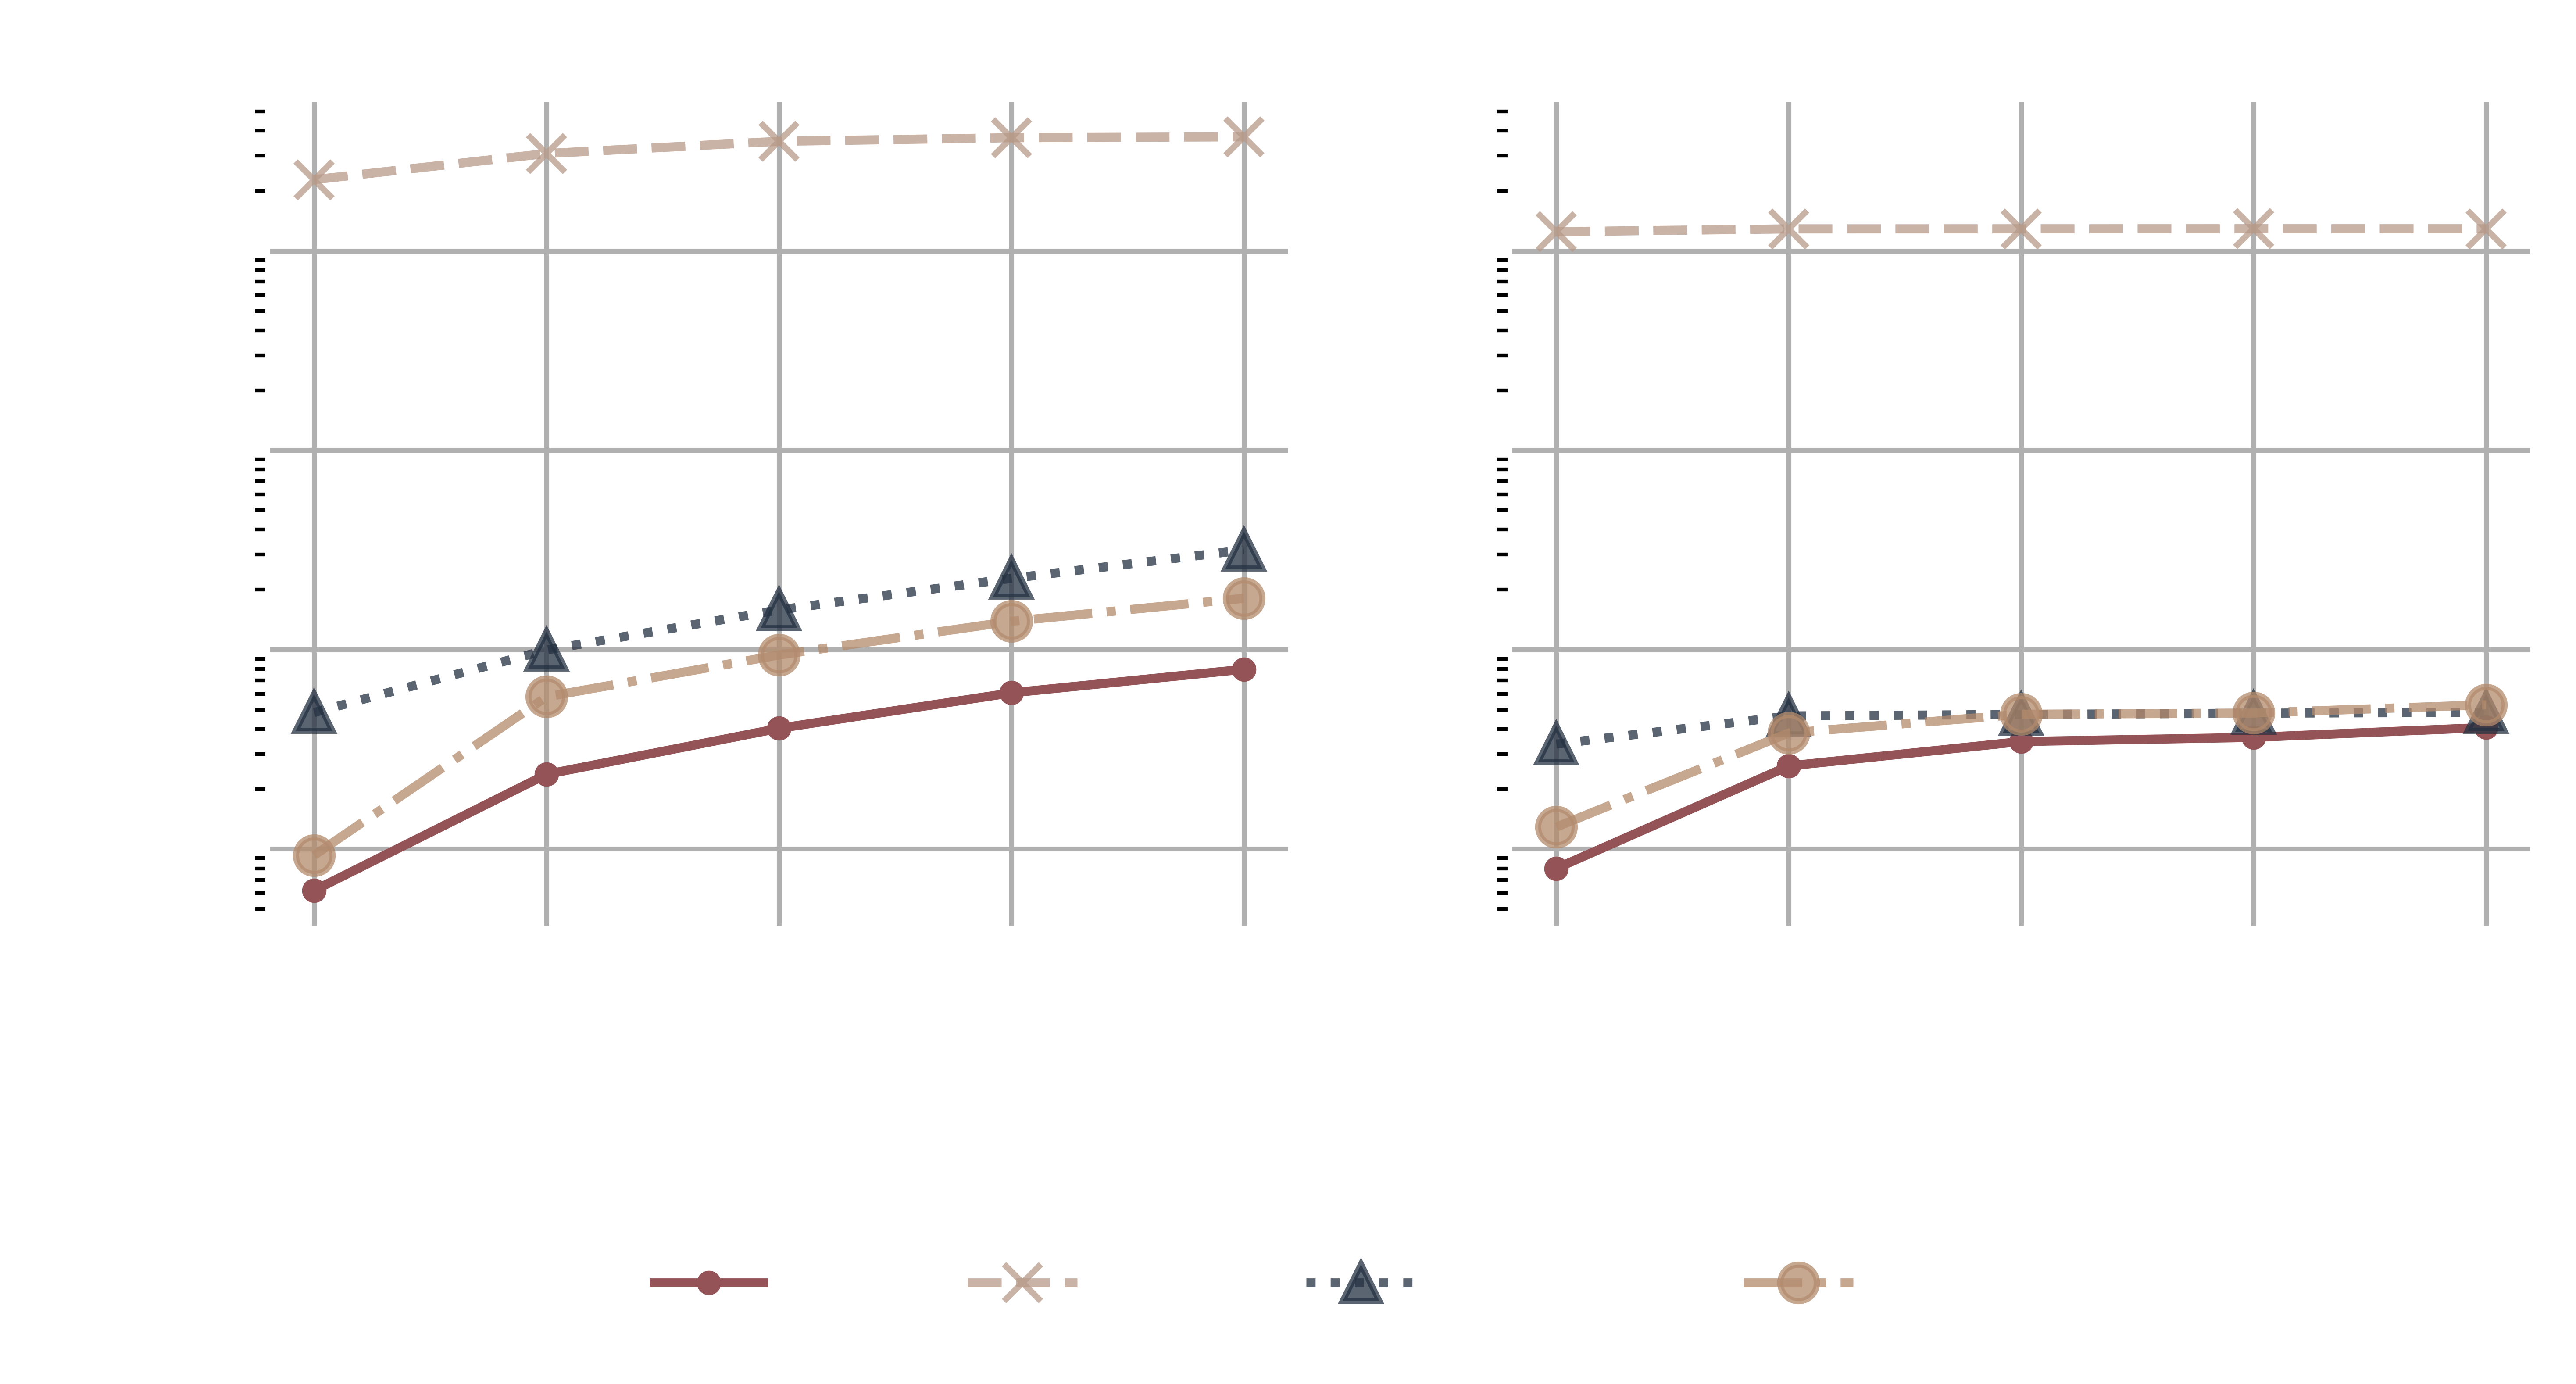
\includegraphics{absolute_performance_2-OAS-GDSW.pdf}
    \caption{Plot of the number of CG iterations $m$ (solid, red line with small circle markers)required to achieve convergence of the solution to \cref{prob:elliptic_problem_discretized} in the sense of criterion \cref{eq:residual_convergence_criterion_r} with $\epsilon_r=10^{-8}$. The left and right columns corresponds to the $\mathcal{C}_{\text{3layer, vert}}$ and $\mathcal{C}_{\text{edge slabs, around vertices}}$ coefficient functions. Also shown are the corresponding classical $m_1$ (dashed, light-gray line with cross markers), multi-cluster $m_{N_{\text{cluster}}}$ (dotted, dark-blue line with triangle markers), and multi-tail-cluster $m_{N_{\text{tail-cluster}}}$ (dash-dotted, gold line with big circle markers) bounds for the CG method applied to the eigenspectra obtained from the Lanczos matrix convergence (Ritz values).}
    \label{fig:cg_bounds_gdsw}
\end{figure}
\begin{figure}[H]
    \centering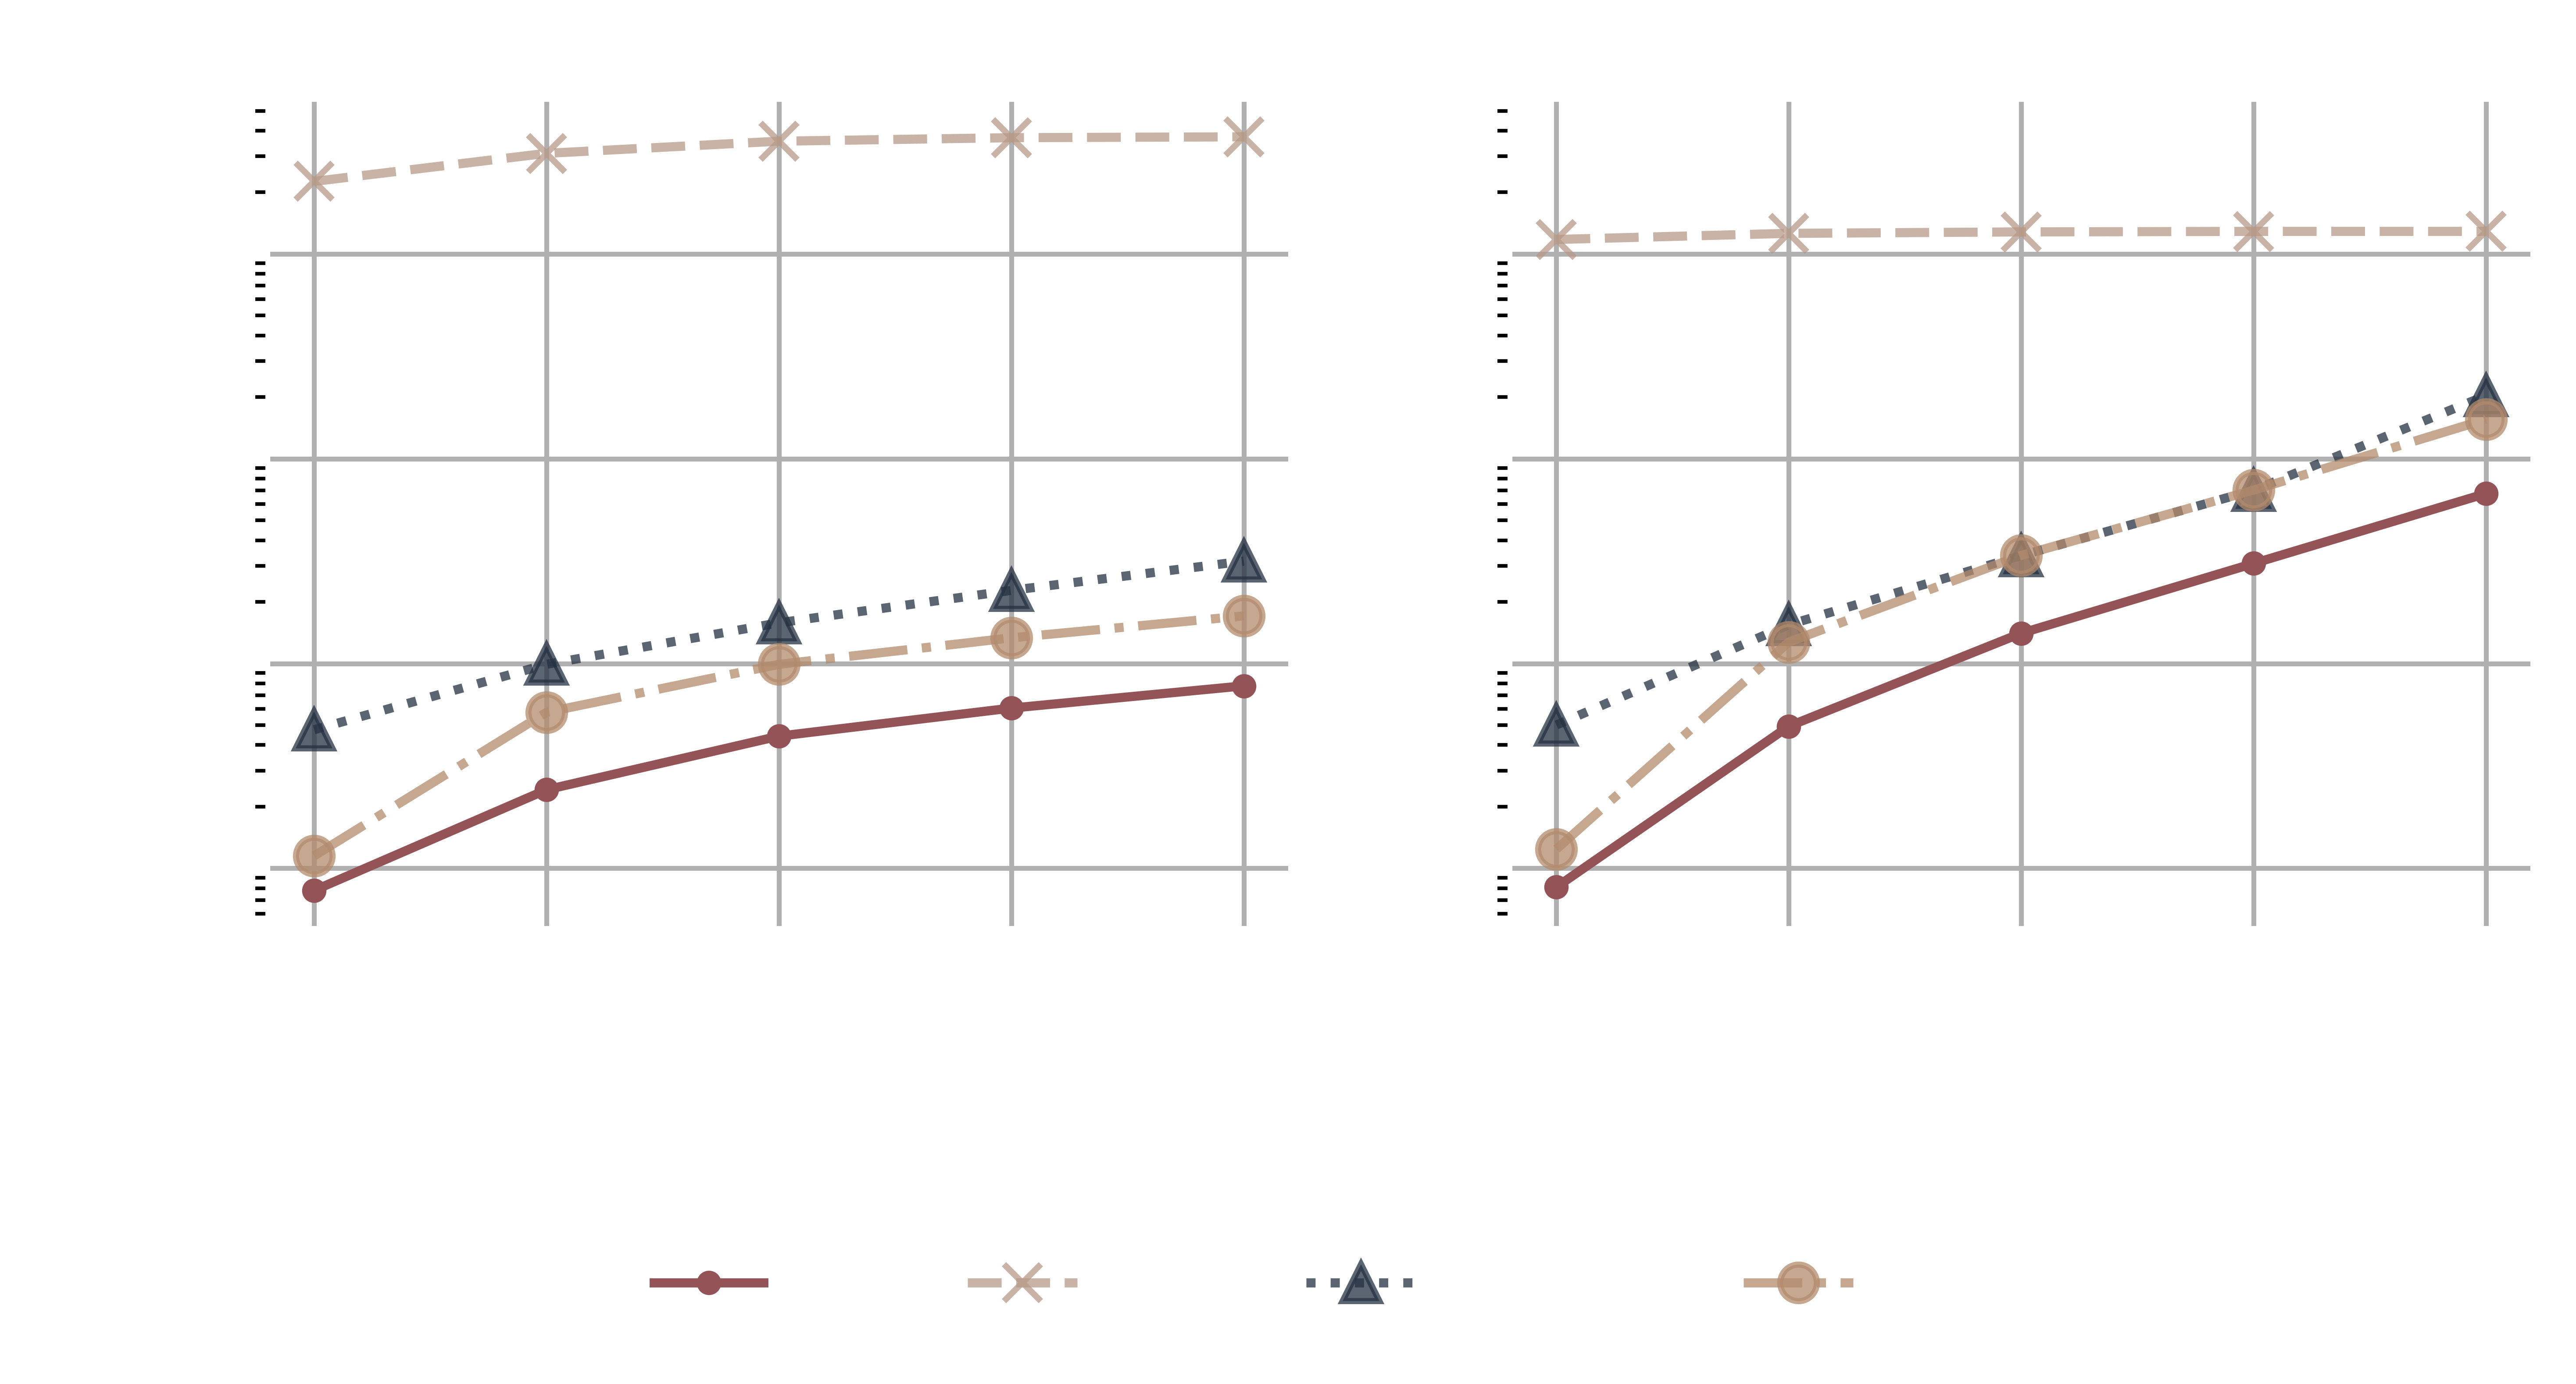
\includegraphics{absolute_performance_2-OAS-RGDSW.pdf}
    \caption{Similar to \cref{fig:cg_bounds_gdsw}, but now for RGDSW coarse space.}
    \label{fig:cg_bounds_rgdsw}
\end{figure}
\begin{figure}[H]
    \centering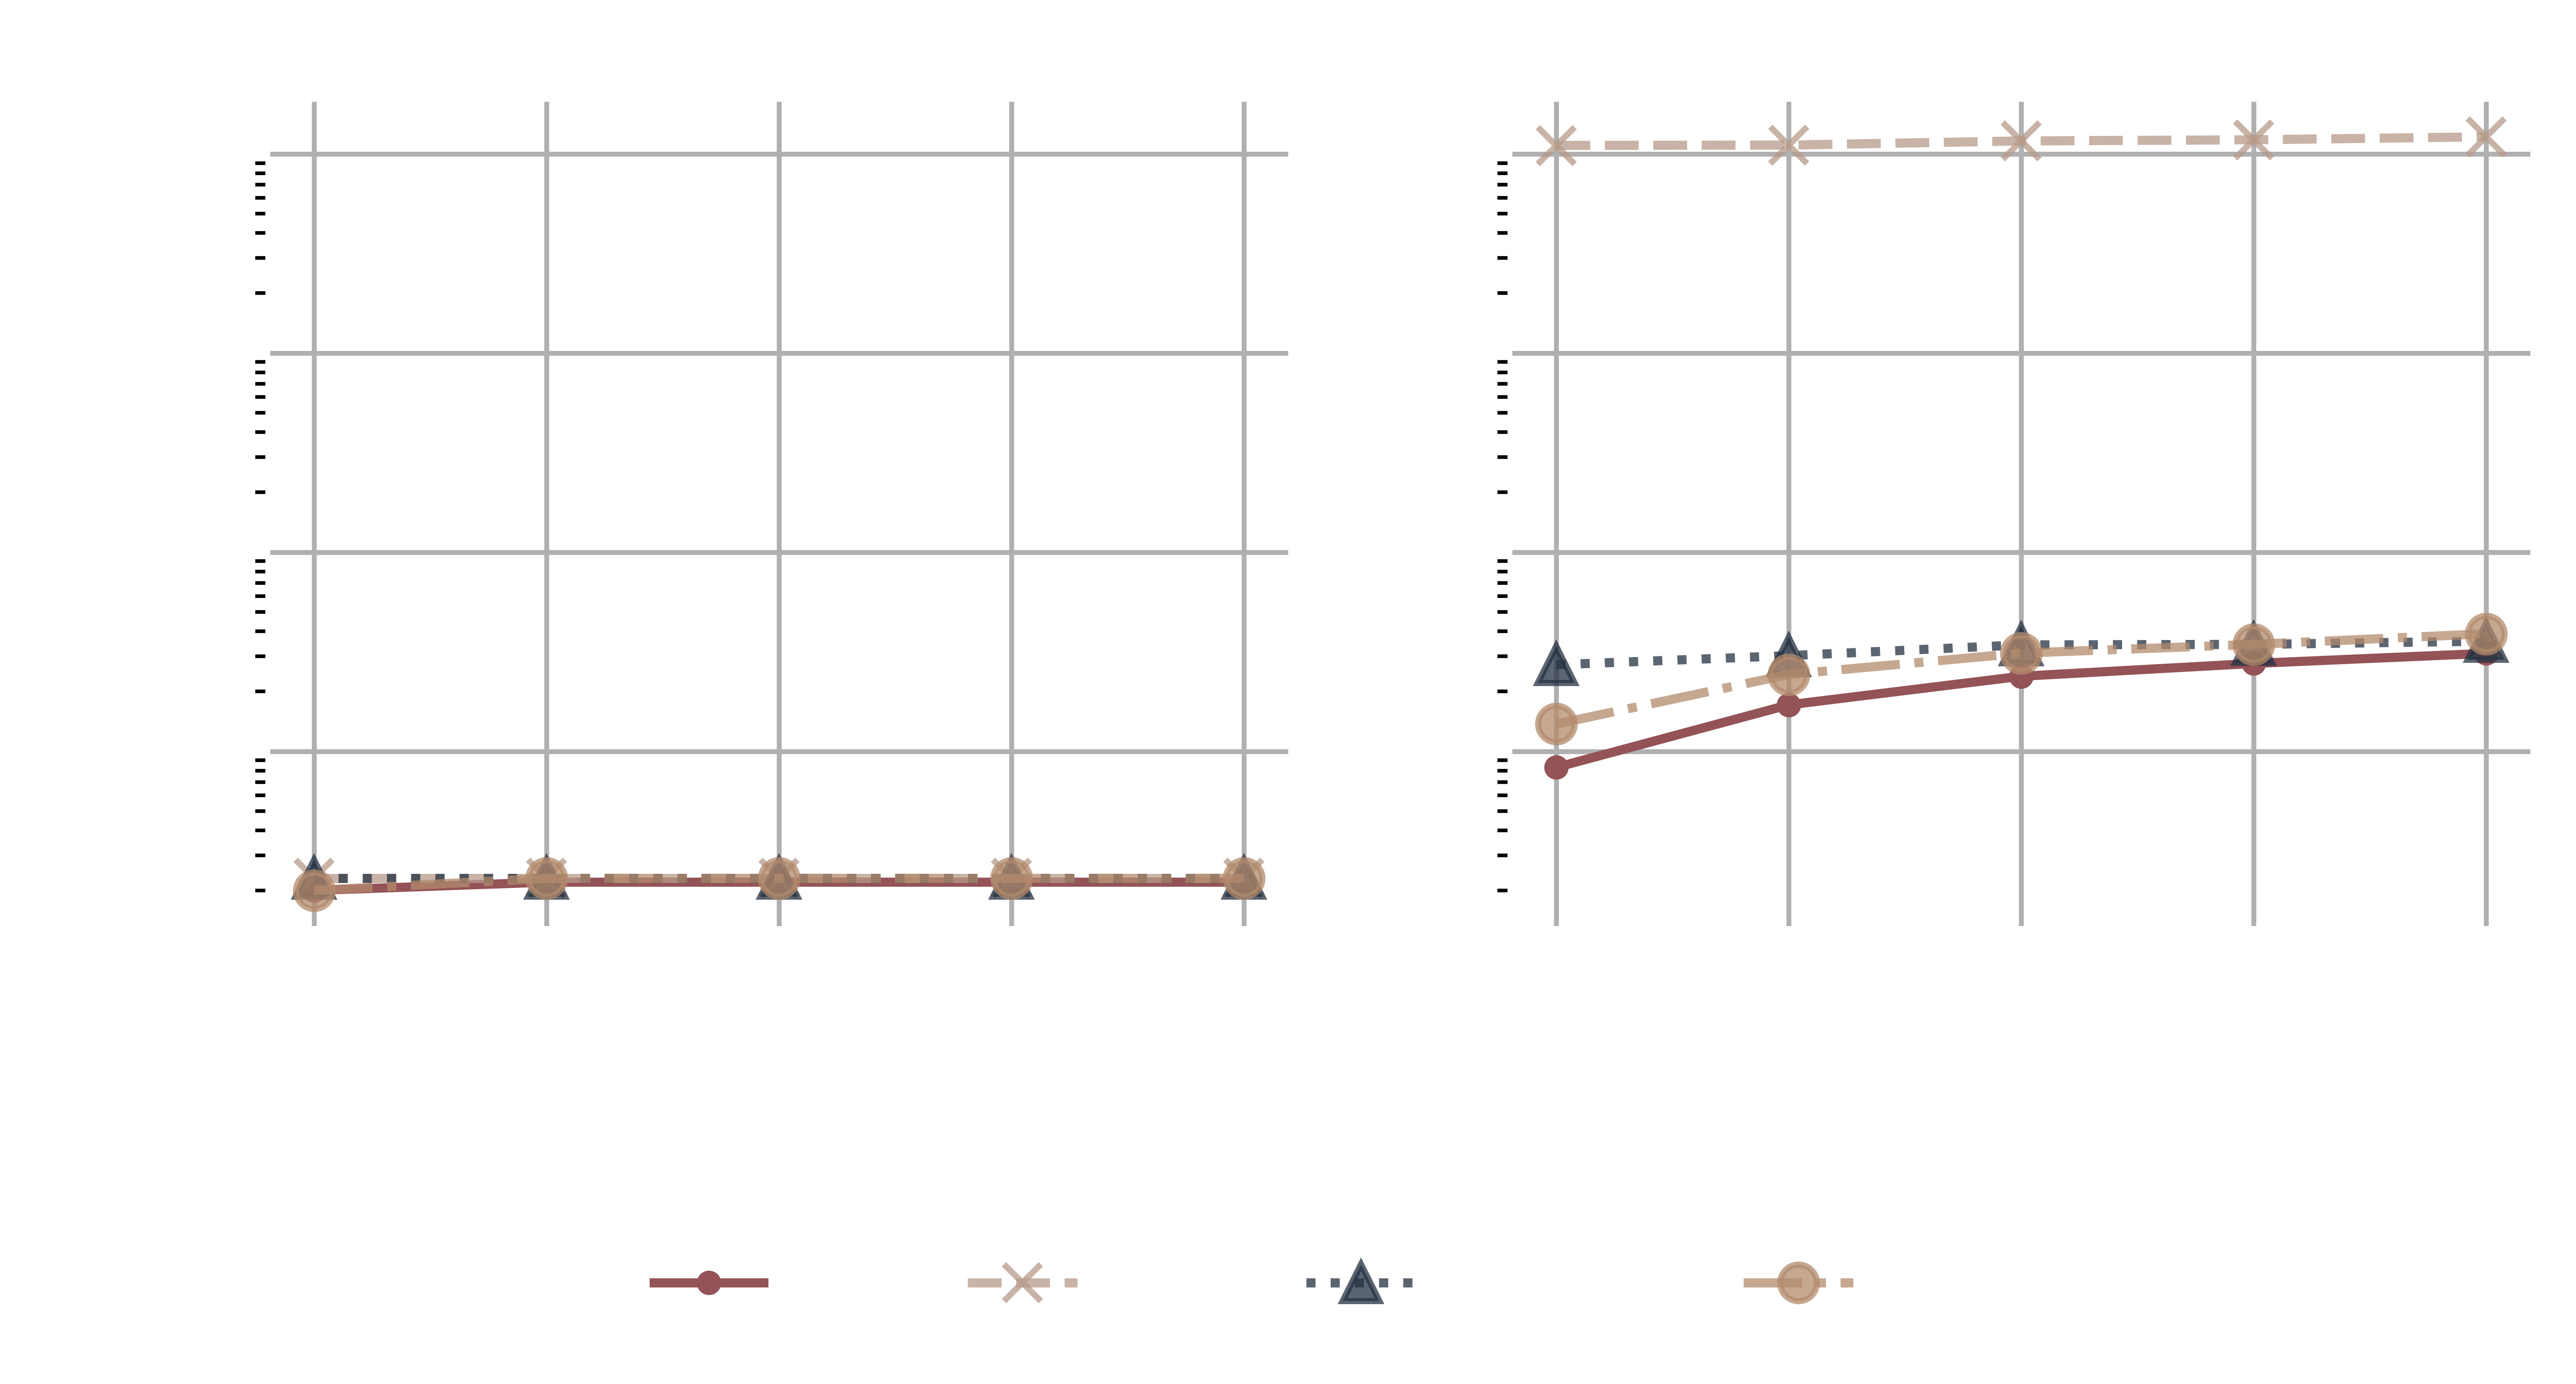
\includegraphics{absolute_performance_2-OAS-AMS.pdf}
    \caption{Similar to \cref{fig:cg_bounds_gdsw}, but now for AMS coarse space.}
    \label{fig:cg_bounds_ams}
\end{figure}
Additionally, it appears $m_{N_{\text{tail-cluster}}} \lesssim m_{N_{\text{cluster}}}$. Even though this was not a design goal of the multi-tail-cluster CG iteration bound, it is a desirable property. The reason for the sharper multi-tail-cluster bound stems from the more rigorous partitioning done by $\operatorname{PartitionEigenspectrumTails}$ compared to $\operatorname{PartitionEigenspectrum}$, as shown in \cref{fig:partitioning_eigenspectrum_tails} and the related discussion above.

\section{Early estimation of CG iteration bounds}\label{sec:early_estimation_of_iterations}
\todo{Add plot of bounds convergence on some high-contrast coefficient function for a robust coarse space (AMS) together with its eigenspectrum. Explain the migration of Ritz values and the fact that we need to wait for temporary convergence of clusters to reliably calculate and update the new bounds.}
\begin{figure}[H]
    \centering
    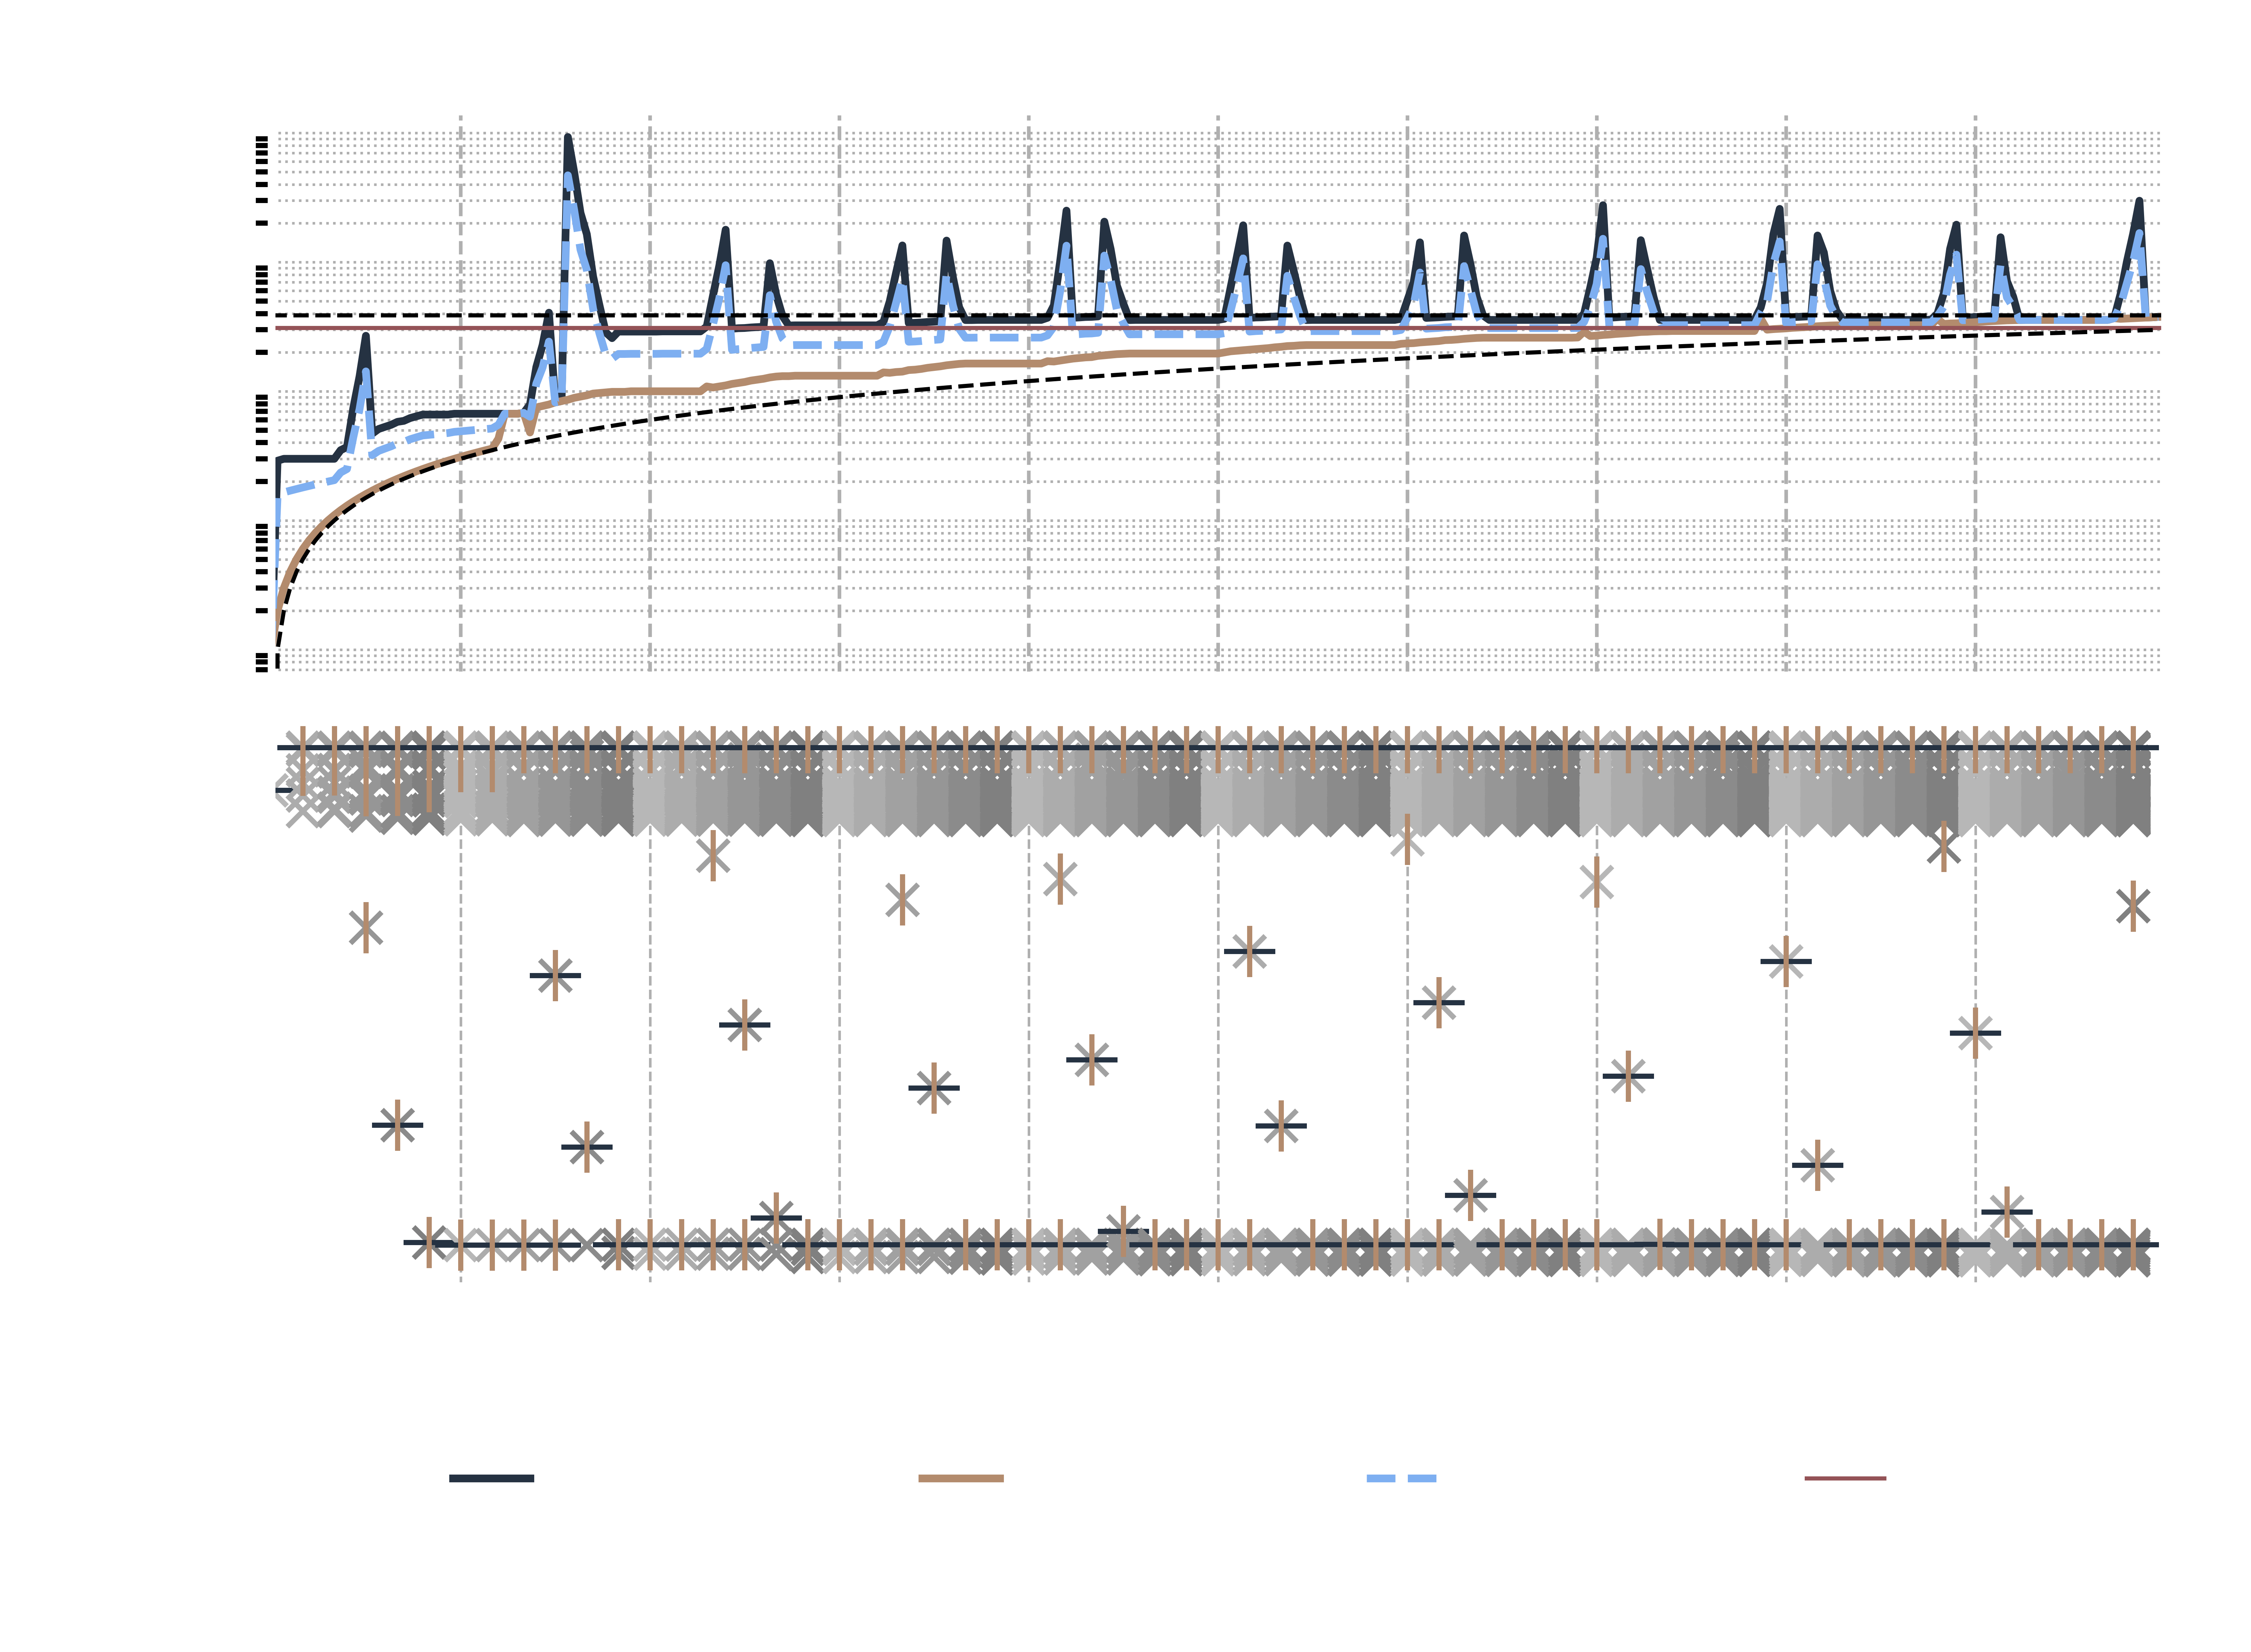
\includegraphics{bound_and_spectrum_vs_iterations_2-OAS-AMS.pdf}
    \caption{}
    \label{fig:bound_and_spectrum_vs_iterations_2-OAS-AMS}
\end{figure}
\begin{figure}[H]
    \centering
    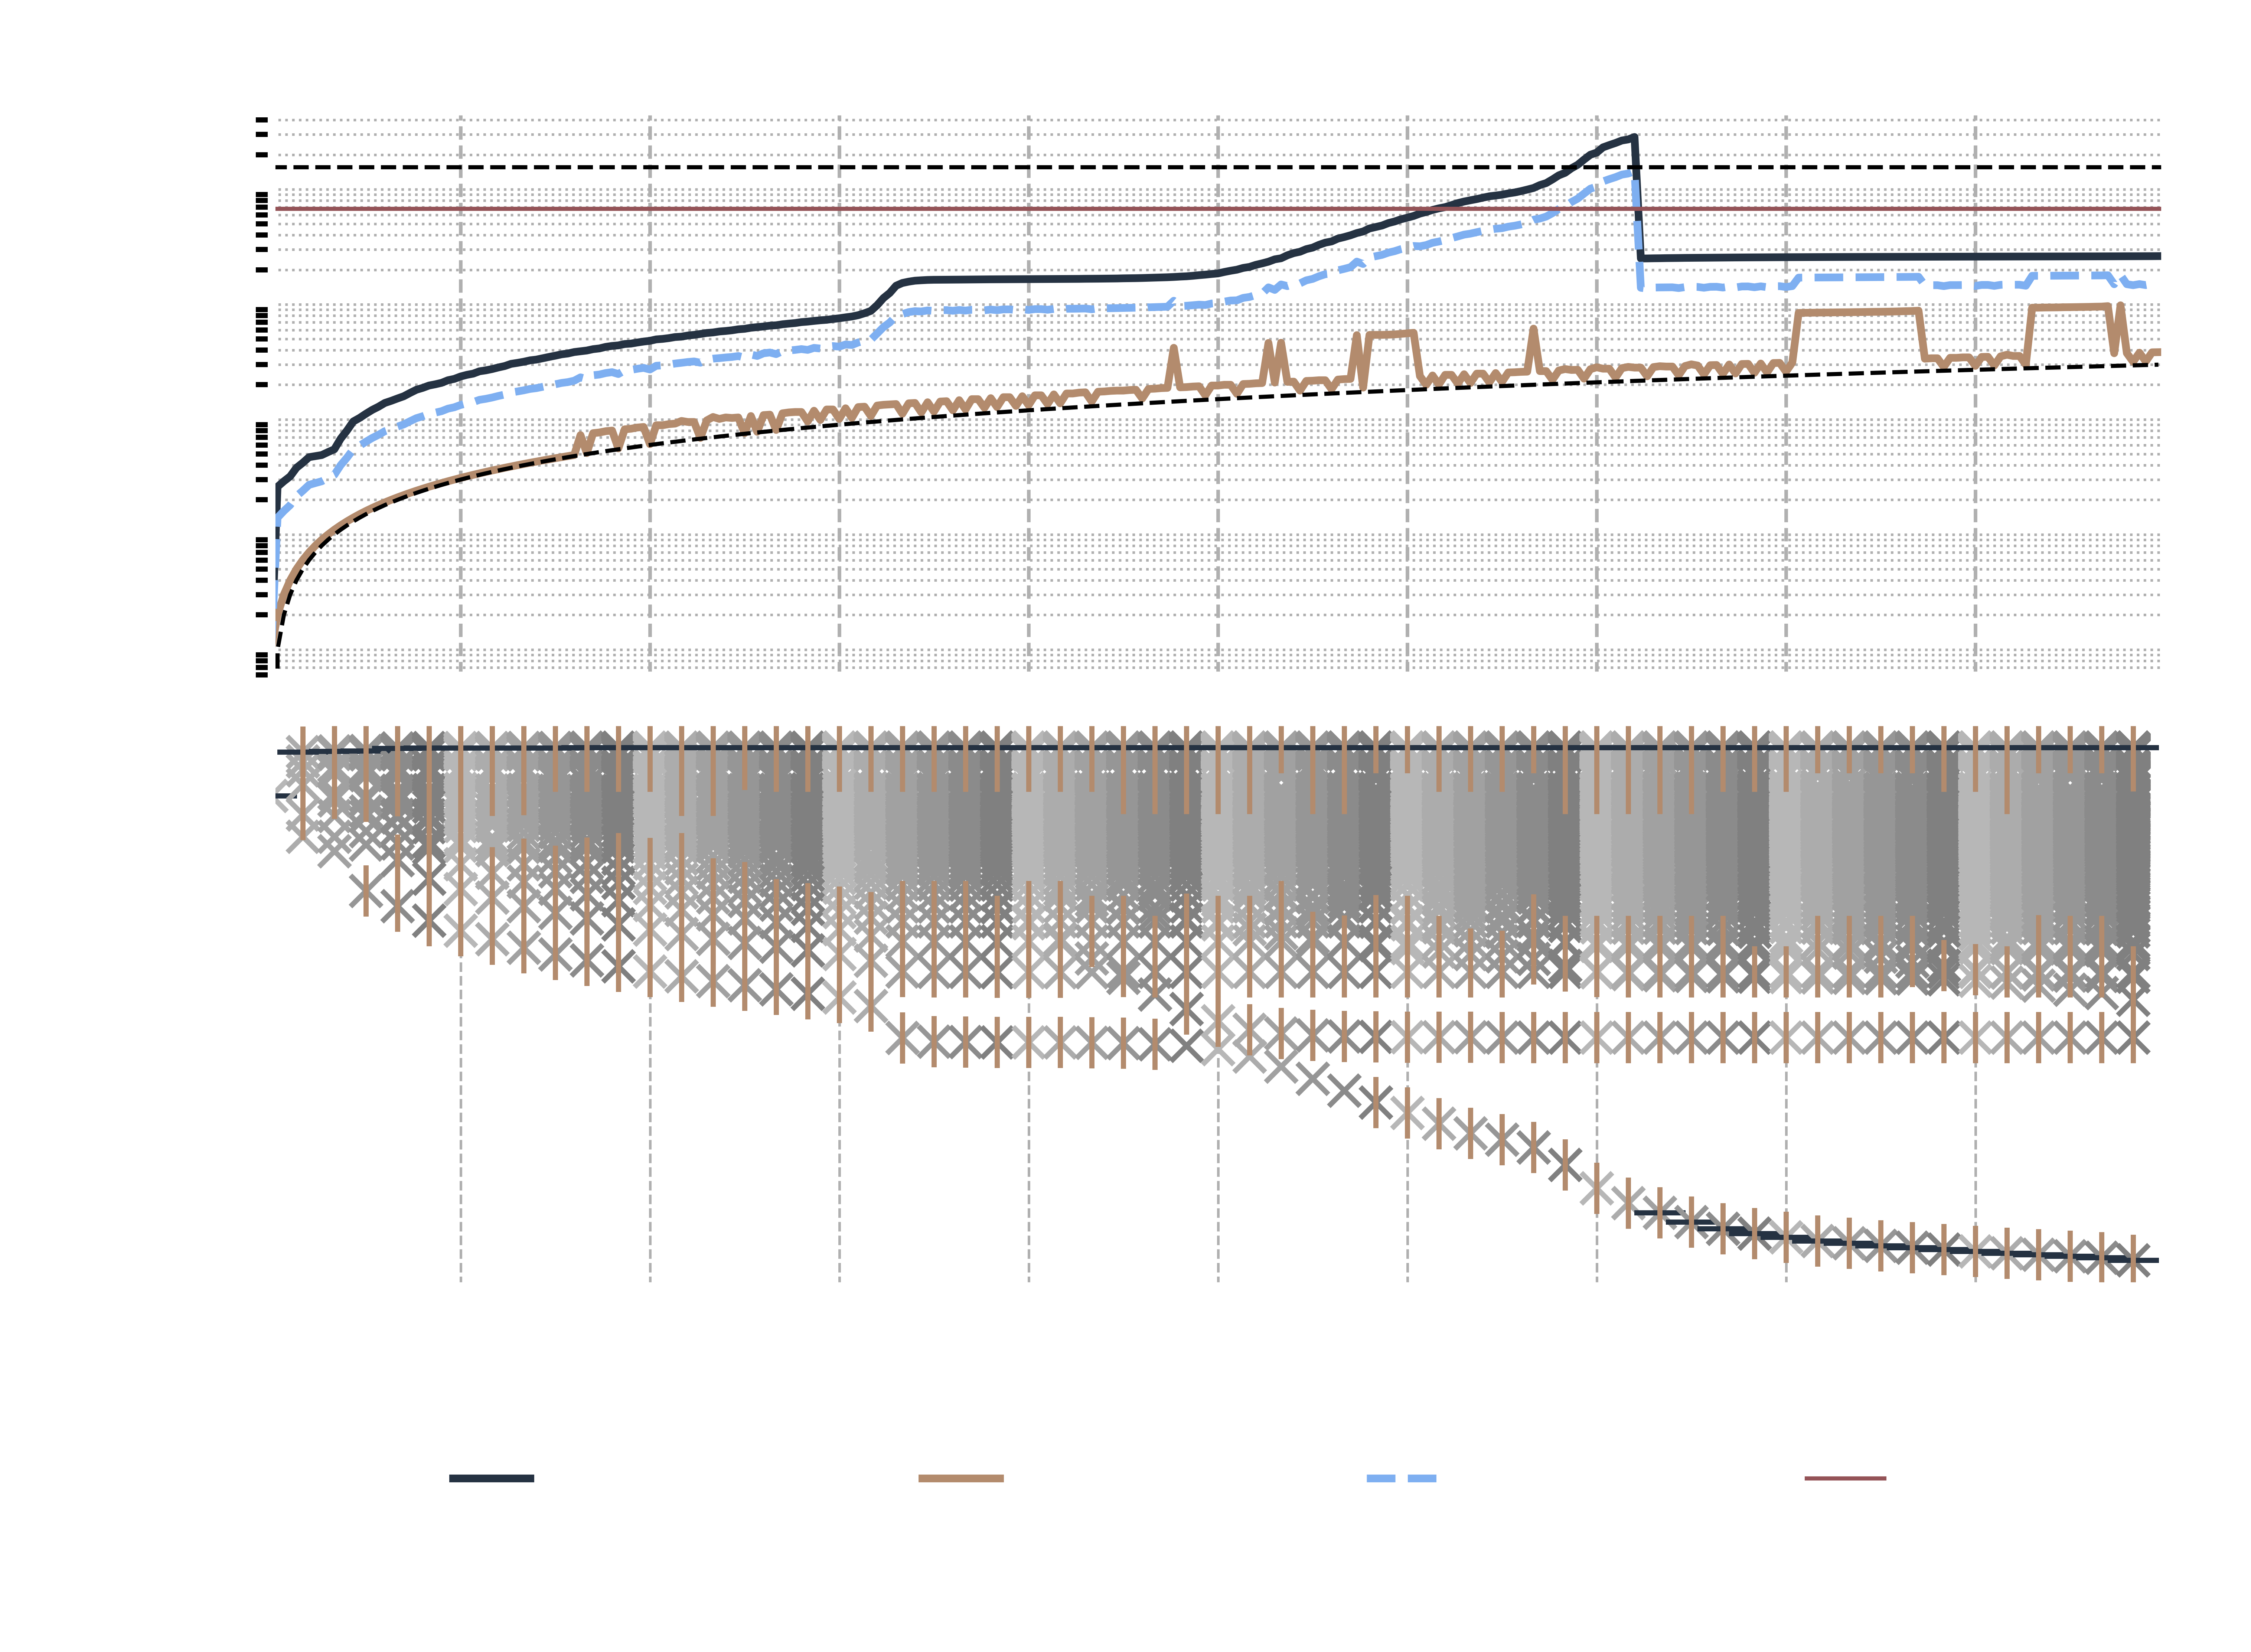
\includegraphics{bound_and_spectrum_vs_iterations_2-OAS-RGDSW.pdf}
    \caption{}
    \label{fig:bound_and_spectrum_vs_iterations_2-OAS-RGDSW}
\end{figure}
\todo{Show the convergence of the RGDSW bound. Ritz value migration happens more slowly so we need more iterations before we can update the bounds.}
\todo{Explain setup of tables}
\begin{table}[H]
\centering
\caption{PCG iteration bounds for solving the model diffusion problem with coefficient function $\mathcal{C}_{\mathrm{const}}$. Bounds are based on approximate spectra (Ritz values) obtained during the initial PCG iterations and are show for meshes $H=1/4$, $H=1/8$, $H=1/16$, $H=1/32$, $H=1/64$ and 2-OAS preconditioners with GDSW, RGDSW, AMS coarse spaces. The $\textbf{bound}$ columns show the values of the CG iteration bounds $m_1$, $m_{N_{\text{cluster}}}$, $m_{N_{\text{tail-cluster}}}$, $m_{\text{estimate}}$ and the $\textbf{iter.}$ columns show the iteration at which those bounds are obtained.}
\label{tab:cg_iteration_bound_coef=const}
\begin{tabular}{llrrrllrrll}
\toprule
 &  & \bfseries $m$ & \multicolumn{2}{|c|}{\bfseries $m_1$} & \multicolumn{2}{|c|}{\bfseries $m_{N_{\text{cluster}}}$} & \multicolumn{2}{|c|}{\bfseries $m_{N_{\text{tail-cluster}}}$} & \multicolumn{2}{|c|}{\bfseries $m_{\text{estimate}}$} \\
 &  &  & bound & iter. & bound & iter. & bound & iter. & bound & iter. \\
\midrule
\multirow[c]{3}{*}{\bfseries $H=1/4$} & GDSW & 23 & {\cellcolor[HTML]{004529}} \color[HTML]{F1F1F1} 34 & 11 & {\cellcolor[HTML]{BCE395}} \color[HTML]{000000} {\cellcolor[HTML]{ADD8E6}} - & - & {\cellcolor[HTML]{379E54}} \color[HTML]{F1F1F1} 34 & 11 & {\cellcolor[HTML]{FFFFE5}} \color[HTML]{000000} {\cellcolor[HTML]{ADD8E6}} - & - \\
\cline{2-11}
\bfseries  & RGDSW & 21 & {\cellcolor[HTML]{BCE395}} \color[HTML]{000000} 40 & 11 & {\cellcolor[HTML]{004529}} \color[HTML]{F1F1F1} {\cellcolor[HTML]{ADD8E6}} - & - & {\cellcolor[HTML]{379E54}} \color[HTML]{F1F1F1} 25 & 11 & {\cellcolor[HTML]{FFFFE5}} \color[HTML]{000000} {\cellcolor[HTML]{ADD8E6}} - & - \\
\cline{2-11}
\bfseries  & AMS & 18 & {\cellcolor[HTML]{BCE395}} \color[HTML]{000000} 23 & 11 & {\cellcolor[HTML]{004529}} \color[HTML]{F1F1F1} {\cellcolor[HTML]{ADD8E6}} - & - & {\cellcolor[HTML]{379E54}} \color[HTML]{F1F1F1} 20 & 11 & {\cellcolor[HTML]{FFFFE5}} \color[HTML]{000000} {\cellcolor[HTML]{ADD8E6}} - & - \\
\cline{1-11} \cline{2-11}
\multirow[c]{3}{*}{\bfseries $H=1/8$} & GDSW & 30 & {\cellcolor[HTML]{BCE395}} \color[HTML]{000000} 37 & 16 & {\cellcolor[HTML]{004529}} \color[HTML]{F1F1F1} {\cellcolor[HTML]{ADD8E6}} - & - & {\cellcolor[HTML]{379E54}} \color[HTML]{F1F1F1} 32 & 16 & {\cellcolor[HTML]{FFFFE5}} \color[HTML]{000000} {\cellcolor[HTML]{ADD8E6}} - & - \\
\cline{2-11}
\bfseries  & RGDSW & 32 & {\cellcolor[HTML]{004529}} \color[HTML]{F1F1F1} 43 & 11 & {\cellcolor[HTML]{BCE395}} \color[HTML]{000000} {\cellcolor[HTML]{ADD8E6}} - & - & {\cellcolor[HTML]{379E54}} \color[HTML]{F1F1F1} 43 & 11 & {\cellcolor[HTML]{FFFFE5}} \color[HTML]{000000} {\cellcolor[HTML]{ADD8E6}} - & - \\
\cline{2-11}
\bfseries  & AMS & 21 & {\cellcolor[HTML]{004529}} \color[HTML]{F1F1F1} 23 & 11 & {\cellcolor[HTML]{BCE395}} \color[HTML]{000000} {\cellcolor[HTML]{ADD8E6}} - & - & {\cellcolor[HTML]{379E54}} \color[HTML]{F1F1F1} 23 & 11 & {\cellcolor[HTML]{FFFFE5}} \color[HTML]{000000} {\cellcolor[HTML]{ADD8E6}} - & - \\
\cline{1-11} \cline{2-11}
\multirow[c]{3}{*}{\bfseries $H=1/16$} & GDSW & 33 & {\cellcolor[HTML]{BCE395}} \color[HTML]{000000} 37 & 16 & {\cellcolor[HTML]{004529}} \color[HTML]{F1F1F1} {\cellcolor[HTML]{ADD8E6}} - & - & {\cellcolor[HTML]{379E54}} \color[HTML]{F1F1F1} 32 & 16 & {\cellcolor[HTML]{FFFFE5}} \color[HTML]{000000} {\cellcolor[HTML]{ADD8E6}} - & - \\
\cline{2-11}
\bfseries  & RGDSW & 38 & {\cellcolor[HTML]{004529}} \color[HTML]{F1F1F1} 45 & 16 & {\cellcolor[HTML]{BCE395}} \color[HTML]{000000} {\cellcolor[HTML]{ADD8E6}} - & - & {\cellcolor[HTML]{379E54}} \color[HTML]{F1F1F1} 28 & 16 & {\cellcolor[HTML]{FFFFE5}} \color[HTML]{000000} {\cellcolor[HTML]{ADD8E6}} - & - \\
\cline{2-11}
\bfseries  & AMS & 22 & {\cellcolor[HTML]{004529}} \color[HTML]{F1F1F1} 24 & 16 & {\cellcolor[HTML]{BCE395}} \color[HTML]{000000} {\cellcolor[HTML]{ADD8E6}} - & - & {\cellcolor[HTML]{379E54}} \color[HTML]{F1F1F1} 24 & 16 & {\cellcolor[HTML]{FFFFE5}} \color[HTML]{000000} {\cellcolor[HTML]{ADD8E6}} - & - \\
\cline{1-11} \cline{2-11}
\multirow[c]{3}{*}{\bfseries $H=1/32$} & GDSW & 35 & {\cellcolor[HTML]{004529}} \color[HTML]{F1F1F1} 37 & 16 & {\cellcolor[HTML]{BCE395}} \color[HTML]{000000} {\cellcolor[HTML]{ADD8E6}} - & - & {\cellcolor[HTML]{379E54}} \color[HTML]{F1F1F1} 28 & 16 & {\cellcolor[HTML]{FFFFE5}} \color[HTML]{000000} {\cellcolor[HTML]{ADD8E6}} - & - \\
\cline{2-11}
\bfseries  & RGDSW & 42 & {\cellcolor[HTML]{004529}} \color[HTML]{F1F1F1} 44 & 16 & {\cellcolor[HTML]{BCE395}} \color[HTML]{000000} {\cellcolor[HTML]{ADD8E6}} - & - & {\cellcolor[HTML]{379E54}} \color[HTML]{F1F1F1} 28 & 16 & {\cellcolor[HTML]{FFFFE5}} \color[HTML]{000000} {\cellcolor[HTML]{ADD8E6}} - & - \\
\cline{2-11}
\bfseries  & AMS & 22 & {\cellcolor[HTML]{004529}} \color[HTML]{F1F1F1} 24 & 16 & {\cellcolor[HTML]{BCE395}} \color[HTML]{000000} {\cellcolor[HTML]{ADD8E6}} - & - & {\cellcolor[HTML]{379E54}} \color[HTML]{F1F1F1} 24 & 16 & {\cellcolor[HTML]{FFFFE5}} \color[HTML]{000000} {\cellcolor[HTML]{ADD8E6}} - & - \\
\cline{1-11} \cline{2-11}
\multirow[c]{3}{*}{\bfseries $H=1/64$} & GDSW & 36 & {\cellcolor[HTML]{004529}} \color[HTML]{F1F1F1} 37 & 16 & {\cellcolor[HTML]{BCE395}} \color[HTML]{000000} {\cellcolor[HTML]{ADD8E6}} - & - & {\cellcolor[HTML]{379E54}} \color[HTML]{F1F1F1} 28 & 16 & {\cellcolor[HTML]{FFFFE5}} \color[HTML]{000000} {\cellcolor[HTML]{ADD8E6}} - & - \\
\cline{2-11}
\bfseries  & RGDSW & 45 & {\cellcolor[HTML]{004529}} \color[HTML]{F1F1F1} 44 & 16 & {\cellcolor[HTML]{BCE395}} \color[HTML]{000000} {\cellcolor[HTML]{ADD8E6}} - & - & {\cellcolor[HTML]{379E54}} \color[HTML]{F1F1F1} 36 & 16 & {\cellcolor[HTML]{FFFFE5}} \color[HTML]{000000} {\cellcolor[HTML]{ADD8E6}} - & - \\
\cline{2-11}
\bfseries  & AMS & 23 & {\cellcolor[HTML]{004529}} \color[HTML]{F1F1F1} 29 & 11 & {\cellcolor[HTML]{BCE395}} \color[HTML]{000000} {\cellcolor[HTML]{ADD8E6}} - & - & {\cellcolor[HTML]{379E54}} \color[HTML]{F1F1F1} 29 & 11 & {\cellcolor[HTML]{FFFFE5}} \color[HTML]{000000} {\cellcolor[HTML]{ADD8E6}} - & - \\
\cline{1-11} \cline{2-11}
\bottomrule
\end{tabular}
\end{table}

\begin{table}[H]
\centering
\caption{PCG iteration bounds $m_1$, $m_{N_{\text{cluster}}}$, $m_{N_{\text{tail-cluster}}}$, $m_{\text{estimate}}$ for solving the model diffusion problem with coefficient function $\mathcal{C}_{\mathrm{3layer, \ vert}}$. Bounds are based on approximate spectra (Ritz values) obtained during the initial PCG iterations and are shown for meshes $\mathbf{H=1/4}$, $\mathbf{H=1/8}$, $\mathbf{H=1/16}$, $\mathbf{H=1/32}$, $\mathbf{H=1/64}$ and 2-OAS preconditioners with GDSW, RGDSW, AMS coarse spaces. The $\textbf{iter.}$ column shows the iteration at which the bounds are obtained.}
\label{tab:cg_iteration_bound_coef=3lvert}
\begin{tabular}{llrrrrrr}
\toprule
 &  & $m$ & $m_1$ & $m_{N_{\text{cluster}}}$ & $m_{N_{\text{tail-cluster}}}$ & $m_{\text{estimate}}$ & \textbf{iter.} \\
\midrule
\multirow[c]{3}{*}{$\mathbf{H=1/4}$} & GDSW & 62 & {\cellcolor[HTML]{E2E4FB}} \color[HTML]{000000} 225,419 & {\cellcolor[HTML]{ACB8F4}} \color[HTML]{000000} 111 & {\cellcolor[HTML]{768BEC}} \color[HTML]{F1F1F1} 26 & {\cellcolor[HTML]{405FE5}} \color[HTML]{F1F1F1} 69 & 26 \\
\cline{2-8}
 & RGDSW & 78 & {\cellcolor[HTML]{E2E4FB}} \color[HTML]{000000} 224,028 & {\cellcolor[HTML]{768BEC}} \color[HTML]{F1F1F1} 109 & {\cellcolor[HTML]{ACB8F4}} \color[HTML]{000000} 26 & {\cellcolor[HTML]{405FE5}} \color[HTML]{F1F1F1} 68 & 26 \\
\cline{2-8}
 & AMS & 20 & {\cellcolor[HTML]{405FE5}} \color[HTML]{F1F1F1} 23 & {\cellcolor[HTML]{405FE5}} \color[HTML]{F1F1F1} 23 & {\cellcolor[HTML]{E2E4FB}} \color[HTML]{000000} 11 & {\cellcolor[HTML]{405FE5}} \color[HTML]{F1F1F1} 17 & 11 \\
\cline{1-8} \cline{2-8}
\multirow[c]{3}{*}{$\mathbf{H=1/8}$} & GDSW & 237 & {\cellcolor[HTML]{E2E4FB}} \color[HTML]{000000} 300,788 & {\cellcolor[HTML]{ACB8F4}} \color[HTML]{000000} 641 & {\cellcolor[HTML]{768BEC}} \color[HTML]{F1F1F1} 91 & {\cellcolor[HTML]{405FE5}} \color[HTML]{F1F1F1} 366 & 51 \\
\cline{2-8}
 & RGDSW & 242 & {\cellcolor[HTML]{E2E4FB}} \color[HTML]{000000} 302,967 & {\cellcolor[HTML]{ACB8F4}} \color[HTML]{000000} 638 & {\cellcolor[HTML]{768BEC}} \color[HTML]{F1F1F1} 86 & {\cellcolor[HTML]{405FE5}} \color[HTML]{F1F1F1} 362 & 51 \\
\cline{2-8}
 & AMS & 22 & {\cellcolor[HTML]{405FE5}} \color[HTML]{F1F1F1} 23 & {\cellcolor[HTML]{405FE5}} \color[HTML]{F1F1F1} 23 & {\cellcolor[HTML]{E2E4FB}} \color[HTML]{000000} 11 & {\cellcolor[HTML]{91A1F0}} \color[HTML]{F1F1F1} 17 & 11 \\
\cline{1-8} \cline{2-8}
\multirow[c]{3}{*}{$\mathbf{H=1/16}$} & GDSW & 403 & {\cellcolor[HTML]{E2E4FB}} \color[HTML]{000000} 350,992 & {\cellcolor[HTML]{ACB8F4}} \color[HTML]{000000} 949 & {\cellcolor[HTML]{768BEC}} \color[HTML]{F1F1F1} 148 & {\cellcolor[HTML]{405FE5}} \color[HTML]{F1F1F1} 549 & 96 \\
\cline{2-8}
 & RGDSW & 442 & {\cellcolor[HTML]{E2E4FB}} \color[HTML]{000000} 351,891 & {\cellcolor[HTML]{ACB8F4}} \color[HTML]{000000} 948 & {\cellcolor[HTML]{768BEC}} \color[HTML]{F1F1F1} 147 & {\cellcolor[HTML]{405FE5}} \color[HTML]{F1F1F1} 548 & 96 \\
\cline{2-8}
 & AMS & 22 & {\cellcolor[HTML]{405FE5}} \color[HTML]{F1F1F1} 23 & {\cellcolor[HTML]{405FE5}} \color[HTML]{F1F1F1} 23 & {\cellcolor[HTML]{E2E4FB}} \color[HTML]{000000} 11 & {\cellcolor[HTML]{91A1F0}} \color[HTML]{F1F1F1} 17 & 11 \\
\cline{1-8} \cline{2-8}
\multirow[c]{3}{*}{$\mathbf{H=1/32}$} & GDSW & 607 & {\cellcolor[HTML]{E2E4FB}} \color[HTML]{000000} 367,021 & {\cellcolor[HTML]{ACB8F4}} \color[HTML]{000000} 2,228 & {\cellcolor[HTML]{405FE5}} \color[HTML]{F1F1F1} 231 & {\cellcolor[HTML]{768BEC}} \color[HTML]{F1F1F1} 1,230 & 161 \\
\cline{2-8}
 & RGDSW & 606 & {\cellcolor[HTML]{E2E4FB}} \color[HTML]{000000} 368,220 & {\cellcolor[HTML]{ACB8F4}} \color[HTML]{000000} 2,277 & {\cellcolor[HTML]{405FE5}} \color[HTML]{F1F1F1} 290 & {\cellcolor[HTML]{768BEC}} \color[HTML]{F1F1F1} 1,284 & 216 \\
\cline{2-8}
 & AMS & 22 & {\cellcolor[HTML]{405FE5}} \color[HTML]{F1F1F1} 23 & {\cellcolor[HTML]{405FE5}} \color[HTML]{F1F1F1} 23 & {\cellcolor[HTML]{E2E4FB}} \color[HTML]{000000} 11 & {\cellcolor[HTML]{91A1F0}} \color[HTML]{F1F1F1} 17 & 11 \\
\cline{1-8} \cline{2-8}
\multirow[c]{3}{*}{$\mathbf{H=1/64}$} & GDSW & 797 & {\cellcolor[HTML]{E2E4FB}} \color[HTML]{000000} 359,087 & {\cellcolor[HTML]{ACB8F4}} \color[HTML]{000000} 1,764 & {\cellcolor[HTML]{768BEC}} \color[HTML]{F1F1F1} 85 & {\cellcolor[HTML]{405FE5}} \color[HTML]{F1F1F1} 925 & 46 \\
\cline{2-8}
 & RGDSW & 778 & {\cellcolor[HTML]{E2E4FB}} \color[HTML]{000000} 359,976 & {\cellcolor[HTML]{ACB8F4}} \color[HTML]{000000} 1,763 & {\cellcolor[HTML]{768BEC}} \color[HTML]{F1F1F1} 85 & {\cellcolor[HTML]{405FE5}} \color[HTML]{F1F1F1} 924 & 51 \\
\cline{2-8}
 & AMS & 22 & {\cellcolor[HTML]{405FE5}} \color[HTML]{F1F1F1} 23 & {\cellcolor[HTML]{405FE5}} \color[HTML]{F1F1F1} 23 & {\cellcolor[HTML]{E2E4FB}} \color[HTML]{000000} 11 & {\cellcolor[HTML]{91A1F0}} \color[HTML]{F1F1F1} 17 & 11 \\
\cline{1-8} \cline{2-8}
\bottomrule
\end{tabular}
\end{table}

\begin{table}[H]
\centering
\caption{PCG iteration bounds for coefficient function $\mathcal{C}_{\mathrm{edge \ slabs, \ around \ vertices}}$ based on approximate spectra (Ritz values) from the first 300 iterations of solving the model diffusion problem on the meshes $H=1/4$, $H=1/8$, $H=1/16$, $H=1/32$, $H=1/64$ using 2-OAS preconditioners with GDSW, RGDSW, AMS coarse spaces. The $\textbf{bound}$ columns show the values of the CG iteration bounds $m_1$, $m_{N_{\text{cluster}}}$, $m_{N_{\text{tail-cluster}}}$, $m_{\text{estimate}}$ and the ($\textbf{iter.}$) column shows the iteration at which these are obtained.}
\label{tab:cg_iteration_bound_Nc64_N=300}
\begin{tabular}{llrrrrrrrrr}
\toprule
 &  & m & \multicolumn{2}{|c|}{$m_1$} & \multicolumn{2}{|c|}{$m_{N_{\text{cluster}}}$} & \multicolumn{2}{|c|}{$m_{N_{\text{tail-cluster}}}$} & \multicolumn{2}{|c|}{$m_{\text{estimate}}$} \\
 &  & \rotatebox{45}{\bfseries } & \rotatebox{45}{\bfseries bound} & \rotatebox{45}{\bfseries iter.} & \rotatebox{45}{\bfseries bound} & \rotatebox{45}{\bfseries iter.} & \rotatebox{45}{\bfseries bound} & \rotatebox{45}{\bfseries iter.} & \rotatebox{45}{\bfseries bound} & \rotatebox{45}{\bfseries iter.} \\
\midrule
\multirow[c]{3}{*}{$H=1/4$} & GDSW & 80 & 124,727 & 36 & 88 & 36 & 88 & 36 & 88 & 36 \\
 & RGDSW & 81 & 117,699 & 36 & 133 & 36 & 61 & 36 & 97 & 36 \\
 & AMS & 83 & 105,144 & 66 & 218 & 66 & 111 & 66 & 165 & 66 \\
\cline{1-11}
\multirow[c]{3}{*}{$H=1/8$} & GDSW & 261 & 127,648 & 96 & 383 & 96 & 173 & 96 & 278 & 96 \\
 & RGDSW & 494 & 124,745 & 186 & 1,274 & 186 & 583 & 186 & 929 & 186 \\
 & AMS & 171 & 110,677 & 71 & 302 & 71 & 123 & 71 & 213 & 71 \\
\cline{1-11}
\multirow[c]{3}{*}{$H=1/16$} & GDSW & 346 & 123,872 & 76 & 306 & 76 & 134 & 76 & 220 & 76 \\
 & RGDSW & 1,406 & 122,195 & 241 & 2,185 & 241 & 979 & 241 & 1,582 & 241 \\
 & AMS & 238 & 110,969 & 81 & 310 & 81 & 126 & 81 & 218 & 81 \\
\cline{1-11}
\multirow[c]{3}{*}{$H=1/32$} & GDSW & 363 & 122,634 & 76 & 310 & 76 & 136 & 76 & 223 & 76 \\
 & RGDSW & 3,082 & 109,007 & 271 & 1,415 & 271 & 920 & 271 & 1,168 & 271 \\
 & AMS & 276 & 116,797 & 191 & 344 & 191 & 251 & 191 & 298 & 191 \\
\cline{1-11}
\multirow[c]{3}{*}{$H=1/64$} & GDSW & 407 & 127,897 & 186 & 485 & 186 & 268 & 186 & 377 & 186 \\
 & RGDSW & 6,766 & 69,645 & 291 & 2,612 & 291 & 956 & 291 & 1,784 & 291 \\
 & AMS & 310 & 120,694 & 196 & 357 & 196 & 260 & 196 & 309 & 196 \\
\cline{1-11}
\bottomrule
\end{tabular}
\end{table}

\todo{Discuss the tables: how many iterations are needed to get a good estimate of the bounds? How do the bounds compare to the classical bound? How do the bounds compare to each other?}